\documentclass{article}
\usepackage[T1]{fontenc}
\usepackage{lmodern}
\usepackage{graphicx}
\usepackage{amsmath,amssymb}
\usepackage[a4paper,margin=2cm]{geometry}
\usepackage[absolute,overlay]{textpos}
\setlength{\TPHorizModule}{1mm}
\setlength{\TPVertModule}{1mm}
\usepackage[indonesian]{babel}
\usepackage{hyperref}
\setlength{\emergencystretch}{2em}
% unit: Halaman 24

\begin{document}

% === Halaman 24 (llm) ===

\vspace{100mm}

\textbf{Gambar Jaringan Feistel di dalam RC6.}\\
Fungsi $f$ adalah $f(x) = x(2x + 1)$ (Rivest, 1998)

% deskripsi: Diagram jaringan Feistel yang digunakan dalam algoritma enkripsi RC6, menunjukkan aliran data melalui beberapa ronde dengan operasi XOR, pergeseran bit (rotate), dan fungsi $f$.
% bbox normalisasi: [0.1200, 0.2000, 0.5300, 0.8400]
\begin{textblock*}{86.10mm}(25.20mm,59.40mm)
\noindent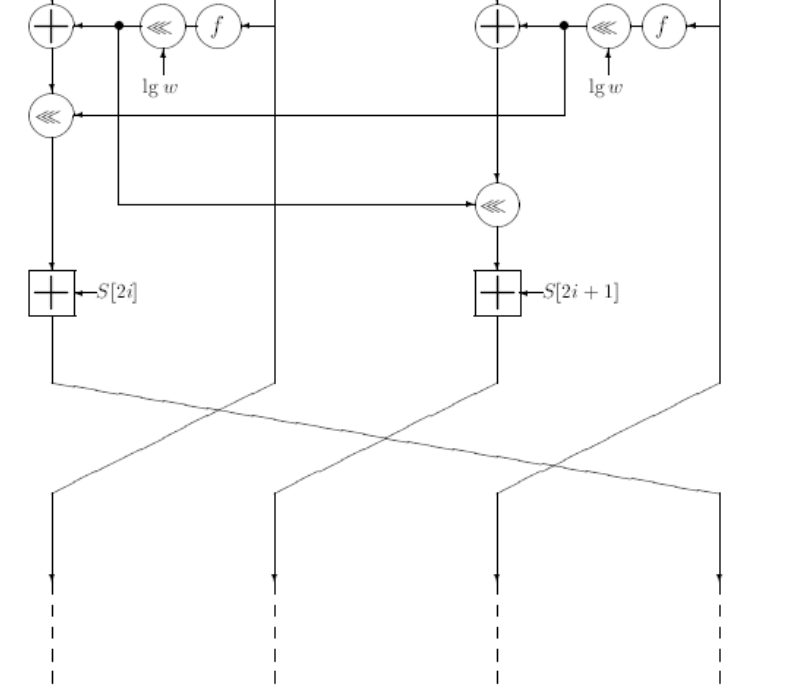
\includegraphics[width=86.10mm,height=190.08mm]{../../images/llm/page_024_img_01.png}%
\end{textblock*}

\end{document}
